\chapter{Численный метод}

\section{Общие положения метода коротких характеристик}
Уравнение \eqref{2} при каждом $\nu$ имеет гиперболический тип и семейство характеристик, которые просто являются характеристиками одномерных уравнений переноса вдоль направления $\vec\Omega$ 
\begin {equation}
\vec r - \vec r_0 = \vec \Omega c(t-t_0).
\end {equation}

Рассмотрим нестационарное уравнение переноса
\begin {equation}
\frac{1}{c}\frac{\partial I_{\nu}}{\partial t} + (\vec\Omega \nabla) I_{\nu} + \varkappa_\nu I_\nu = \varkappa_{\nu} I_{\nu p}.
\end {equation}

Выберем некоторым образом на единичной сфере набор направлений $\Theta = \{\vec\omega_i\}_1^n$. Для каждого направления уравнение является одномерным уравнением переноса, причем между собой уравнения не связаны:
\begin {equation}
\begin {cases}
\dfrac{1}{c} \dfrac{\partial I_{\nu,1}}{\partial t} + (\vec\omega_1 \nabla) I_{\nu,1} + \varkappa_\nu I_{\nu,1} = \varkappa_{\nu} I_{\nu p}, \\[12pt]
\dfrac{1}{c} \dfrac{\partial I_{\nu,2}}{\partial t} + (\vec\omega_2 \nabla) I_{\nu,2} + \varkappa_\nu I_{\nu,2} = \varkappa_{\nu} I_{\nu p},\\
\hspace{7,65em}\vdots \\
\dfrac{1}{c} \dfrac{\partial I_{\nu,n}}{\partial t} + (\vec\omega_n \nabla) I_{\nu,n} + \varkappa_\nu I_{\nu,n} = \varkappa_{\nu} I_{\nu p}.
\label {9}
\end {cases}
\end {equation}
С набором направлений $\Theta$ можно связать квадратурную формулу для сферы:
\begin {equation}
\int f(\vec\Omega)d\Omega \approx \sum_{i=1}^n w_i f(\vec \omega_i)
\end {equation}
Соответственно, моменты интенсивности $U, \vec S$ можно определить как
\begin {equation}
U_\nu = \sum_{i=1}^n w_i I_{\nu,i}, \quad
\vec S_\nu = \sum_{i=1}^n w_i \vec \omega_i I_{\nu,i}.
\end {equation}

Неопределенность касается выбора направлений $\Theta$ и численного метода решения каждого уравнения \eqref{9}.

Предположим, что в области решения задачи построена тетраэдральная сетка.
Пусть неизвестная функция интенсивности задана на гранях тетраэдра. В каждом тетраэдре решается уравнение переноса вдоль характеристики точно в предположении, что свойства вещества в тетраэдре постоянны \ref{fig:3}. 

\begin{figure}[ht!]
\centering{
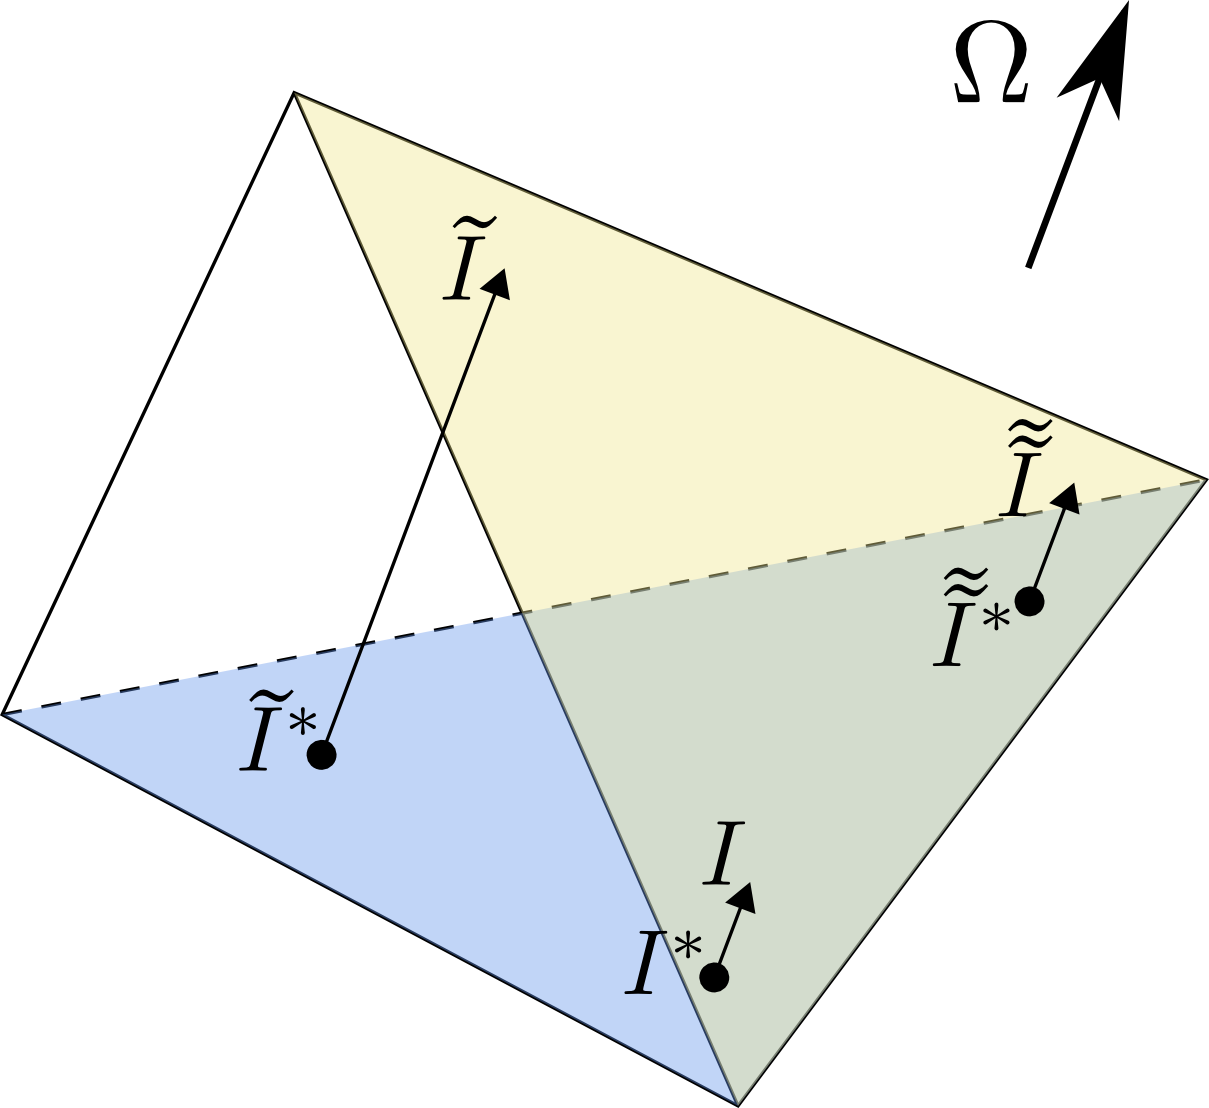
\includegraphics[width = 0.5\textwidth]{slide72.png}
}
\caption{К построению метода коротких характеристик}
\label{fig:3}
\end{figure}

Каждое из уравнений \eqref{8} является гиперболическим и для его решения можно применить сеточно-характеристический метод. Для вычисления интенсивности $I_{\nu,i}$ в точке $p$ выпускается луч в направлении $-\vec\omega_i$ до пересечения с первой гранью. В точке пересечения $\vec r^*$ вычисляется интерполированное по вершинам грани значение интенсивности $I_{\nu, i} (\vec r^*) = \sum_{j = q,r,s} \alpha_jI_{\nu, i}(\vec r_j)$. Далее, $I_{\nu, i} (\vec r_p)$ вычисляется из решения одномерного уравнения переноса   
\begin {equation}
I_{\nu}(s) = \int_{s_0}^s\varkappa'_{\nu}I_{\nu p} \exp\Big[-\int_{s'}^s\varkappa'_{\nu}ds''\Big]ds' + I_{\nu,0} \exp\Big[-\int_{s_0}^s \varkappa'_{\nu}ds''\Big].
\end {equation}

В простом случае, если в тетраэдре $\varkappa_\nu = \operatorname{const}$, формула упрощается до 
\begin {equation}
I_\nu (s) = I_{\nu p} \left(1 - e^{-\varkappa_\nu \Delta}\right) + I_{\nu,0}e^{-\varkappa_\nu \Delta},
\end {equation}
где $\Delta = s - s_0$. Очевидно, что $I_\nu(s)$ лежит в пределах от $I_{\nu, 0}$ до $I_{\nu p}$
\section {Многогрупповое приближение}
Разобъем весь спектр на конечное число $N_k$ интервалов по частоте - групп. Внутри каждой группы для частот $\nu$, лежащих в пределах $\nu_k \leqslant \nu \leqslant \nu_{k+1}$, $\nu_1 = 0$, $\nu_{N_k} = \infty$, будем предполагать, что коэффициент поглощения не зависит от энергии фотона:
\begin {equation}
\varkappa_\nu (T, \rho, \nu) = \varkappa_k(t, \rho), \quad \nu_k \leqslant \nu \leqslant \nu_{k+1}, \quad k = 1 \div N_k.
\label{10}
\end {equation}
Интегральный потом и плотность энергии излучения представим в виде
\begin {equation}
\vec W = \int_0^\infty d\nu \int \vec\Omega I_\nu d\Omega = \sum_{k=1}^{N_k} \int \vec\Omega I_k d\Omega, \quad I_k = \int_{\nu_k}^{\nu_{k+1}} I_\nu d \nu, 
\end {equation}
\begin {equation}
U = \frac{1}{c} \int_0^\infty d\nu \int I_\nu d \Omega = \sum_{k=1}^{N_k} \frac{1}{c} \int I_k d \Omega.
\end {equation}
Для определения уравнения, которому удовлетворяет $I_k$, проинтегрируем уравнение переноса по $\nu$ от $\nu_k$ до $\nu_{k+1}$. Учитывая, что коэффициент поглощения \eqref{10} в этом диапазоне не зависит от частоты, получим
\begin {equation}
(\vec\Omega \nabla )I_k + \varkappa_k I_k = \varkappa_k \int_{\nu_k}^{\nu_{k+1}} I_{\nu, p} d \nu.
\end {equation}
Многогрупповое приближение позволяет рассматривать уравнение переноса как уравнение относительно вектор-функции $\vec I $ интенсивности излучения, компоненты которой являются значением интенсивности в своей частотной группе. 
После преобразования уравнения \eqref{2} получим
\begin {equation}
(\vec\Omega \nabla ) \vec I + \vec K \vec I = \vec K \vec I_{p},
\end {equation}
где $\vec K = diag \varpkappa_k$. Если рассматривать это уравнение как векторное, то можно избежать повторения одинаковых геометрических вычислений для каждой частоты.
\section{Маршевый метод}
Разделим грани тетраэдра на входящие и выходящие \ref{fig:4}. Грань называется входящей, если луч, пересекающий ее, входит в тетраэдр, в противном случае~--- выходящей. Решение на выходящих гранях тетраэдра можно найти только тогда, когда решение на входящих гранях уже посчитано. Соответственно, на гранях триангуляции образуется отношение частичного порядка. В случае, если это отношение не образует цикл, его можно распространить на все множество граней, то есть задать такой порядок обхода граней, при котором выходные грани каждого тетраэдра идут после входных граней этого же тетраэдра. 

\begin{figure}[ht!]
\centering{
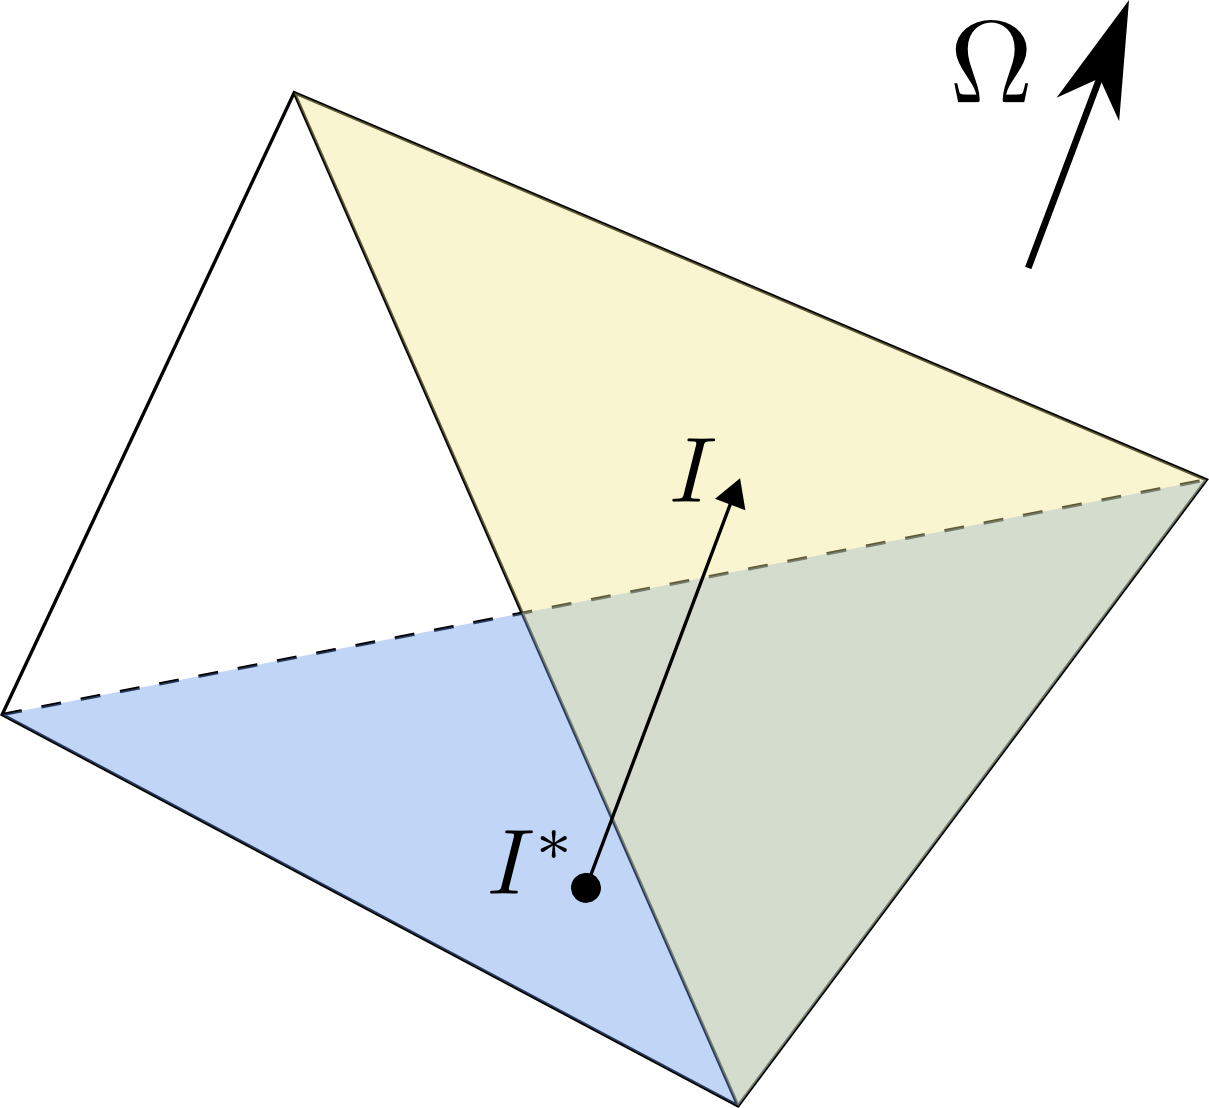
\includegraphics[width = 0.7\textwidth]{slide71.png}
}
\caption{Входящие и выходящие грани тетраэдра.}
\label{fig:4}
\end{figure}

Для триангуляции Делоне порядок, в котором свет проходит грани такой же, в котором свет проходит центры описанных вокруг тетраэдра сфер, и требуемый порядок можно получить сортировкой координат центров тетраэдров вдоль направления переноса излучения \cite{skalko_2014}.

В случае, если триангуляция не является триангуляцией Делоне, такая сортировка может привести к неверному результату: могут образоваться тетраэдры, в которых выходные грани проходятся раньше входных. Однако задача упорядочения граней решается для более широкого класса, чем класс триангуляций Делоне. 

Предлагается следующий алгоритм упорядочения, являющийся адаптацией поиска в ширину. Частичный порядок граней порождает отношение порядка тетраэдров. Нужно пометить тетраэдры номером так, чтобы отношение порядка было связано соответственно с возрастанием номера тетраэдра. Пусть $c(T)$ - номер (цвет) тетраэдра $T$. Тогда условие упорядоченности можно записать как $ c(T) > c (T')$ для всех $T'$, граничащих с $T$ по входной грани. 

Есть очередь тетраэдров, из которой извлекаются и в которую добавляются тетраэдры. В очереди сначала находятся все тетраэдры, грани которых были освещены. За шаг алгоритма из очереди извлекается один тетраэдр, проверяется, все ли его входящие грани освещены. В этом случае тетраэдр удаляется из очереди, а в очередь добавляются все его неосвещенные соседи. Если это не так, тетраэдр добавляется в конец очереди. При работе с очередью производится проверка на цикл: если обнаруживается, что из очереди нельзя удалить ни один тетраэдр, значит, в триангуляции имеется цикл, и алгоритм останавливается (дальнейшее использование маршевого метода невозможно).

Кроме самого упорядочения этот алгоритм группирует грани, решения на которых могут быть вычислены параллельно в силу своей независимости друг от друга. Это может стать основой для последующего распараллеливания алгоритма.
\section{Особенности выбора точек на грани}
Точки, из которых выпускаются характеристики на грани, не могут быть взяты произвольно. Рассмотрим данный метод, примененный к одномерному не стационарному уравнению переноса.

\begin {equation}
\frac{\partial u}{\partial t} + \frac{\partial u}{\partial x} = 0
\end {equation}

На каждом ребре решение является линейной функцией $u_i^n(x) = \alpha_i^nx+\beta_i^n $. Со слоя $n+1$ на $n$ выпускаются две характеристики, на которых решение сохраняется. На слое $n+1$ решается система относительно $\alpha_i^{n+1}$ и $\beta_i^{n+1}$. 

\begin{figure}[ht!]
\centering{
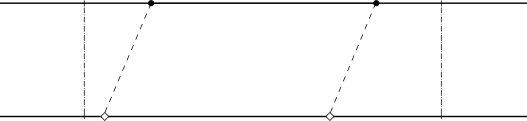
\includegraphics[width = 0.5\textwidth]{bad_char.png}
}
\caption{Положение характеристик при $\sigma < \sigma_\text{кр}$}
\label{fig:5}
\end{figure}
Числом Куранта для этой задачи будет $\tau/h$, а $\sigma_\text{кр} = h_1/h$. Когда число Куранта $\sigma < \sigma_\text{кр}$, схема теряет устойчивость, так как решение не может покинуть ячейку (см. рис. \ref{fig:5}). Такого эффекта нет, если характеристики выпускаются из узлов расчетной сетки. Он проявляется на прямоугольных сетках, неизвестно, какой эффект он окажет на неструктурированные. В связи с этим в используемом методе в набор точек, из которых испускается характеристики, всегда включаются вершины граней. 
\section{Повышение порядка пространственной аппроксимации. Монотонная интерполяция}
В случае использования минимального количества (трех вершин на каждой грани), получается метод первого порядка, который имеет существенную численную диффузию луча. Получается схема первого порядка, чтобы увеличить точность схемы, используются дополнительные точки на гранях. В качестве таких точек выбираются середины ребер. 

Использование интерполяции на гранях по шести точкам позволяет поднять порядок аппроксимации метода коротких характеристик до второго. Такая параболическая интерполяция имеет существенный недостаток: она не является монотонной, то есть потенциально может приводить к появлению отрицательных значений интенсивности, что лишено физического смысла  \ref{8}. Для того, чтобы избежать немонотонной интерполяции, нужно использовать процедуру ограничения решения в серединах ребер, исходя из соображения, что экстремум параболы должен находиться либо в вершинах ребра, либо за его пределами. 
\begin{figure}[ht!]
	\centering{
		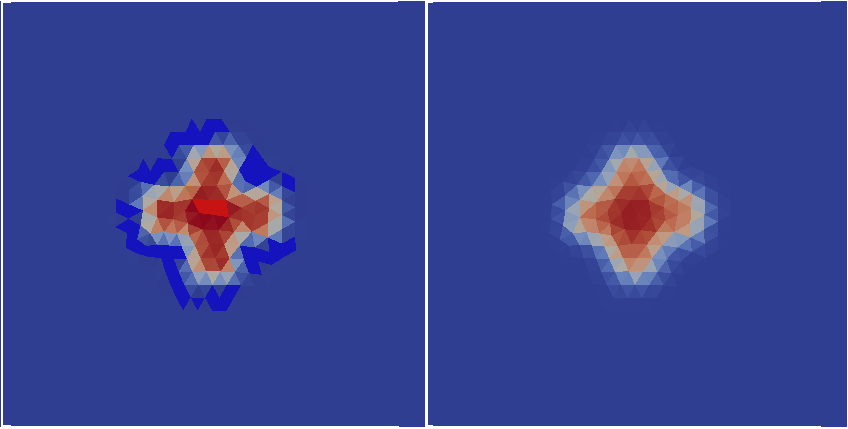
\includegraphics[width = 0.5\textwidth]{2vs2lim.png}
	}
	\caption{Сравнение методов второго порядка и второго с ограничителем}
	\label{fig:8}
\end{figure}
Для этого рассмотрим отрезок $[-1, 1]$. Предполагается, что значение в концах отрезка известны и равны соотвественно $I_1$ и $I_2$. Решение в центре обозначим как $I_{mid}$. Из условия на экстремум следует, что абсцисса вершины параболы должна удовлетворять условию $|x_{\text{верш}}| \geqslant 1 $. Учитывая, что парабола в общем виде $ax^2 + bx + c = 0$ и с нашими условиями имеет следующие коэффициенты:
\begin {equation}
a = \frac{I_1 + I_2 - 2I_{mid}}{2}, \quad b = \frac{I_2 - I_1}{2}, \quad c = I_{mid}, 
\end {equation}
а $x_{\text{верш}} = -\frac{b}{2a}$, получим, что
\begin {equation}
\left| \frac{I_1 - I_2}{2(I_1 + I_2 - 2I_{mid})}\right| \geqslant 1,
\end {equation}
откуда элементарными преобразованиями получаем условие на центр ребра:
\begin {equation}
\left| I_{mid} - \frac{I_1 + I_2}{2}\right| \leqslant \left| \frac{I_1 - I_2}{4}\right| .
\end {equation}
При $a=0$ парабола становится прямой, у нее нет экстремума, следовательно, полученное условие будет верно. 
В численном методе значение интенсивности на ребрах ограничиваются по ближайшей границе допустимого интервала. Для выявления разницы между схемами первого и второго порядка аппроксимации использовались также кусочно-линейная интерполяция интенсивности по шести точкам. Это позволяет сравнить метод первого и второго порядка при одинаковом количестве (степеней свободы) узловых точек. 

В качестве базиса для квадратичной интерполяции используются функции $\ell_0 \div \ell_5$, которые в стандартном треугольнике  имеют вид:

\begin {equation}
\begin {aligned}
\ell_0 (\xi, \eta)&= (\eta + \xi -1)(2\eta + 2\xi - 1) \\
\ell_1 (\xi, \eta)&= \xi(2\xi - 1) \\
\ell_2 (\xi, \eta)&= \eta (2\eta - 1) \\
\ell_3 (\xi, \eta)&= 4\eta\xi \\
\ell_4 (\xi, \eta)&= -4\eta(\eta + \xi - 1) \\
\ell_5 (\xi, \eta)&= -4\xi(\eta + \xi - 1) \\
\end {aligned}
\end {equation}

Для интерполяции первого порядка для тех же шести точек используются следующие базисные функции:

\begin {equation}
\begin {aligned}
\ell_0 (\xi, \eta) &= 
\begin{cases}
0, & \xi + \eta \geqslant 0.5 \\
1-2(\xi + \eta), & \xi + \eta < 0.5
\end{cases}
 \\
\ell_1 (\xi, \eta) = \ell_2 (\eta, \xi) &= 
\begin{cases}
0, & \xi < 0.5 \\
2\xi - 1, & \xi > 0.5
\end{cases}
\\
\ell_3 (\xi, \eta) &=
\begin{cases}
0, & \xi + \eta < 0.5 \\
2\eta, & \xi > 0.5 \\
2\xi, &\eta > 0,5 \\
2\xi + 2\eta - 1, & \text{иначе}
\end{cases}
\\
\ell_4 (\xi, \eta) = \ell_5(\eta, \xi)&= 
\begin{cases}
2\eta, & \xi + \eta < 0.5 \\
0, & \xi > 0.5 \\
-2\xi -2\eta + 2, &\eta > 0,5 \\
-2\xi + 1, & \text{иначе}
\end{cases}
\\
\end {aligned}
\end {equation}

Причем, для случая первого порядка коррекция значений на ребрах не требуется.